\documentclass[10pt,a4paper,twocolumn,twoside]{article}
\usepackage[utf8]{inputenc}
\usepackage[catalan]{babel}
\usepackage{multicol}
\usepackage{graphicx}
\usepackage{fancyhdr}
\usepackage{times}
\usepackage{titlesec}
\usepackage{multirow}
\usepackage{lettrine}
\usepackage[top=2cm, bottom=1.5cm, left=2cm, right=2cm]{geometry}
\usepackage[figurename=Fig.,tablename=TAULA]{caption}
\captionsetup[table]{textfont=sc}

\author{\LARGE\sffamily Nom de l'estudiant}
\title{\Huge{\sffamily Títol de l'Article (màxim 3 línies)}}
\date{}

\newcommand\blfootnote[1]{%
  \begingroup
  \renewcommand\thefootnote{}\footnote{#1}%
  \addtocounter{footnote}{-1}%
  \endgroup
}

%
%\large\bfseries\sffamily
\titleformat{\section}
{\large\sffamily\scshape\bfseries}
{\textbf{\thesection}}{1em}{}

\begin{document}

\fancyhead[LO]{\scriptsize AUTOR: TÍTOL DEL TREBALL}
\fancyhead[RO]{\thepage}
\fancyhead[LE]{\thepage}
\fancyhead[RE]{\scriptsize EE/UAB TFG INFORMÀTICA: TÍTOL (ABREUJAT SI ÉS MOLT LLARG)}

\fancyfoot[CO,CE]{}

\fancypagestyle{primerapagina}
{
   \fancyhf{}
   \fancyhead[L]{\scriptsize TFG EN ENGINYERIA INFORMÀTICA, ESCOLA D'ENGINYERIA (EE), UNIVERSITAT AUTÒNOMA DE BARCELONA (UAB)}
   \fancyfoot[C]{\scriptsize ``Mes'' de 20xx, Escola d'Enginyeria (UAB)}
}

%\lhead{\thepage}
%\chead{}
%\rhead{\tiny EE/UAB TFG INFORMÀTICA: TÍTOL (ABREUJAT SI ÉS MOLT LLARG)}
%\lhead{ EE/UAB \thepage}
%\lfoot{}
%\cfoot{\tiny{February 2015, Escola d'Enginyeria (UAB)}}
%\rfoot{}
\renewcommand{\headrulewidth}{0pt}
\renewcommand{\footrulewidth}{0pt}
\pagestyle{fancy}

%\thispagestyle{myheadings}
\twocolumn[\begin{@twocolumnfalse}

%\vspace*{-1cm}{\scriptsize TFG EN ENGINYERIA INFORMÀTICA, ESCOLA D'ENGINYERIA (EE), UNIVERSITAT AUTÒNOMA DE BARCELONA (UAB)}

\maketitle

\thispagestyle{primerapagina}
%\twocolumn[\begin{@twocolumnfalse}
%\maketitle
%\begin{abstract}
\begin{center}
\parbox{0.915\textwidth}
{\sffamily
\textbf{Resum--}
Resum del projecte, màxim 10 línies. ........ ........... .......... ..  ... ..... .... ........ ........... .......... ..  ... ..... .... ........ ........... .......... ..  ... ..... .... ........ ........... .......... ..  ... ..... .... ........ ........... .......... ..  ... ..... .... ........ ........... .......... ..  ... ..... .... ........ ........... .......... ..  ... ..... .... ........ ........... .......... ..  ... ..... .... ........ ........... .......... ..  ... ..... .... ........ ........... .......... ..  ... ..... .... ........ ........... .......... ..  ... ..... .... .................. ..  ... ..... .... ........ ........... .......... ..  ... ..... .... ........ ........... .......... ..  ... ..... .... ........ ........... .......... ..  ... ..... .... ........ ........... .......... ..  ... ..... .... ........ ........... .......... ..  ... ..... .... ........ ........ .......... ..  ... . ........... .......... ..  ... ..... .... ........ ........... .......... ..  ... ..... .... ........ ........... .......... ..  ... ..... .... ........ ........... .......... ..  ... ........... ..  ... ..... .... ........ ........... .......... ..  ... ..... .... ........ ........... .......... ..  ... ..... .... ........ ........... .......... ..  ... ..... .... ........ ........... .......... ..  ... ..... .... ........ ........... .......... ..  ... ..... .... ........ ........... .......... ..  ... ..... .... ........ ........... .......... ..  ... ..... .... ........ ........... .......... ..  ... ..... .... 
\\
\\
\textbf{Paraules clau-- } Paraules clau del treball, màxim 2 línies . .... ........ ........... .......... ..  ... ..... .... ........ ........... .......... ..  ... ..... .... ........ ........... ................\\
\\
%\end{abstract}
%\bigskip
%\begin{abstract}
\bigskip
\\
\textbf{Abstract--} Versió en anglès del resum . ........ ........... .......... ..  ... ..... .... ........ ........... .......... ..  ... ..... .... ........ ........... .......... ..  ... ..... .... ........ ........... .......... ..  ... ..... .... ........ ........... .......... ..  ... ..... .... ........ ........... .......... ..  ... ..... .... ........ ........... .......... ..  ... ..... .... ........ ........... .......... ..  ... ..... .... ........ ........... .......... ..  ... ..... .... ........ ........... .......... ..  ... ..... .... ........ ........... .......... ..  ... ..... .... .................. ..  ... ..... .... ........ ........... .......... ..  ... ..... .... ........ ........... .......... ..  ... ..... .... ........ ........... .......... ..  ... ..... .... ........ ........... .......... ..  ... ..... .... ........ ........... .......... ..  ... ..... .... ........ ........ .......... ..  ... . ........... .......... ..  ... ..... .... ........ ........... .......... ..  ... ..... .... ........ ........... .......... ..  ... ..... .... ........ ........... .......... ..  ... ........... ..  ... ..... .... ........ ........... .......... ..  ... ..... .... ........ ........... .......... ..  ... ..... .... ........ ........... .......... ..  ... ..... .... ........ ........... .......... ..  ... ..... .... ........ ........... .......... ..  ... ..... .... ........ ........... .......... ..  ... ..... .... ........ ........... .......... ..  ... ..... .... ........ ........... .......... ..  ... ..... .... 
\\
\\
\textbf{Keywords-- } Versió en anglès de les paraules clau. .... ........ ........... .......... ..  ... ..... .... ........ ........... .......... ..  ... ..... .... ........ ........... .................. ..\\
}

\bigskip

{\vrule depth 0pt height 0.5pt width 4cm\hspace{7.5pt}%
\raisebox{-3.5pt}{\fontfamily{pzd}\fontencoding{U}\fontseries{m}\fontshape{n}\fontsize{11}{12}\selectfont\char70}%
\hspace{7.5pt}\vrule depth 0pt height 0.5pt width 4cm\relax}

\end{center}

\bigskip
%\end{abstract}
\end{@twocolumnfalse}]

\blfootnote{$\bullet$ E-mail de contacte: xxx@yyy.zzz}
\blfootnote{$\bullet$ Menció realitzada: Enginyeria de Computadors / Computació / Enginyeria del Software / Tecnologies de la Informació}
\blfootnote{$\bullet$ Treball tutoritzat per: nom i cognoms del tutor (departament)}
\blfootnote{$\bullet$ Curs 20xx/xx}

\section{Introducció - Context del treball}

\lettrine[lines=3]{A}{quest} document és una adaptació  de l'estil dels articles de la IEEE i assumeix la utilització de LaTeX. Acompanyant a aquest document podeu trobar l'original en anglès (IEEE-Template) amb les instruccions referents a l'estil. Es recomana llegir el document original per tal de saber com inserir figures i taules, peus de pàgina, equacions, referències, etc. Si us plau, respecteu l'estil i no canvieu la mida de la font, l'espai entre línies, ni la doble columna.

Des del punt de vista del TFG hi ha un límit en el nombre de pàgines: 

\begin{itemize}
\item de 8 a 10 pàgines d’explicació del treball, agraïments i bibliografia.
\item 4 pàgines addicionals per incloure matèria d’apèndix.
\end{itemize}

L'organització en seccions dependrà de cada treball, però de manera genèrica podem esperar:

\begin{itemize}
\item Secció d’introducció on s’explica el context del treball i les motivacions i es plantegen els objectius. També s’explica breument l’organització de la resta del document.
\item Una sèrie de seccions que dependran del treball particular.
\item Una secció on es presenti el mètode d’avaluació dels resultats, els resultats en si mateixos, i una discussió/reflexió sobre aquests resultats.
\item Una secció de conclusió del treball, apuntant també les línies de continuació.
\item Uns petits agraïments, si s’escau.
\item La bibliografia.
\item Una secció a mode d’apèndix, si s’escau.
\end{itemize}

\section{Exemple de Secció}

Això és un exemple de secció que conté dues subseccions (\ref{subsec-exemple1} i \ref{subsec-exemple2}) i una figura (\ref{fig-exemple}).

\subsection{Exemple de subsecció}
\label{subsec-exemple1}

.... ..  .... .. .... ... ..... ... ..... ... ... ..... .... .


% Per a fer que la figura ocupi les dues columnes utilitzeu "figure*" per comptes de "figure"
\begin{figure}[!h]
\centering
	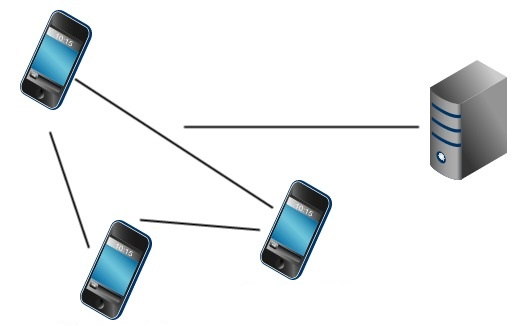
\includegraphics[width=0.4\textwidth]{img/adhoc_dtn}
	\caption{Exemple de figura}
	\label{fig-exemple}
\end{figure}

\subsection{Un altre exemple de subsecció}
\label{subsec-exemple2}

La taula \ref{tab:senzilla} és un exemple de taula senzilla. En canvi, la taula \ref{tab:taula2} és més completa.

Hi ha moltes referències \textit{on-line} de \LaTeX, com \cite{latex}.

% Utilitzeu el begin table només en cas de vole taules flotants. Si les voleu al lloc, tabular directament.
\begin{table}
\caption{Taula d'exemple}
\label{tab:senzilla}
\begin{center}
\begin{tabular}{|c|c|}
\hline
One & Two\\
\hline
Three & Four\\
\hline
\end{tabular}
\end{center}
\end{table}



\begin{table}
\caption{Taula més completa}
\label{tab:taula2}

\begin{center}
\begin{tabular}{ |l|l|l| }
\hline
\multicolumn{3}{ |c| }{Team sheet} \\
\hline
Goalkeeper & GK & Paul Robinson \\ \hline
\multirow{4}{*}{Defenders} & LB & Lucus Radebe \\
 & DC & Michael Duburry \\
 & DC & Dominic Matteo \\
 & RB & Didier Domi \\ \hline
\multirow{3}{*}{Midfielders} & MC & David Batty \\
 & MC & Eirik Bakke \\
 & MC & Jody Morris \\ \hline
Forward & FW & Jamie McMaster \\ \hline
\multirow{2}{*}{Strikers} & ST & Alan Smith \\
 & ST & Mark Viduka \\
\hline
\end{tabular}
\end{center}
\end{table}

\section{Conclusions}

.... ..  .... .. .... ... ..... ... ..... ... ... ..... .... .
.... ..  .... .. .... ... ..... ... ..... ... ... ..... .... .
.... ..  .... .. .... ... ..... ... ..... ... ... ..... .... .
.... ..  .... .. .... ... ..... ... ..... ... ... ..... .... .
.... ..  .... .. .... ... ..... ... ..... ... ... ..... .... .
.... ..  .... .. .... ... ..... ... ..... ... ... ..... .... .
.... ..  .... .. .... ... ..... ... ..... ... ... ..... .... .
.... ..  .... .. .... ... ..... ... ..... ... ... ..... .... .
.... ..  .... .. .... ... ..... ... ..... ... ... ..... .... .
.... ..  .... .. .... ... ..... ... ..... ... ... ..... .... .
.... ..  .... .. .... ... ..... ... ..... ... ... ..... .... .
.... ..  .... .. .... ... ..... ... ..... ... ... ..... .... .
.... ..  .... .. .... ... ..... ... ..... ... ... ..... .... .
.... ..  .... .. .... ... ..... ... ..... ... ... ..... .... .

\section*{Agraïments}

... ..  .... .. .... ... ..... ... ..... ... ... ..... .... .
.... ..  .... .. .... ... ..... ... ..... ... ... ..... .... .
.... ..  .... .. .... ... ..... ... ..... ... ... ..... .... .
.... ..  .... .. .... ... ..... ... ..... ... ... ..... .... .
.... ..  .... .. .... ... ..... ... ..... ... ... ..... .... .

\begin{thebibliography}{11}
\bibitem{latex}
http://en.wikibooks.org/wiki/LaTeX

\bibitem{2}
Referència 2

\bibitem{3}
Etc.


\end{thebibliography}

\appendix

\section*{Apèndix}

\setcounter{section}{1}

\subsection{Secció d'Apèndix}


... ..  .... .. .... ... ..... ... ..... ... ... ..... .... .
.... ..  .... .. .... ... ..... ... ..... ... ... ..... .... .
.... ..  .... .. .... ... ..... ... ..... ... ... ..... .... .
.... ..  .... .. .... ... ..... ... ..... ... ... ..... .... .
.... ..  .... .. .... ... ..... ... ..... ... ... ..... .... .

\subsection{Secció d'Apèndix}


... ..  .... .. .... ... ..... ... ..... ... ... ..... .... .
.... ..  .... .. .... ... ..... ... ..... ... ... ..... .... .
.... ..  .... .. .... ... ..... ... ..... ... ... ..... .... .
.... ..  .... .. .... ... ..... ... ..... ... ... ..... .... .
.... ..  .... .. .... ... ..... ... ..... ... ... ..... .... .


\end{document}

